En counting ADC bruker en binærteller for å \emph{'nærme seg'} riktig verdi.
Binærtelleren tikker høyere og høyere helt til komperatoren bekrefter at
man har funnet høy nok verdi.

En klokke brukes for å samkjøre det hele.

\marginpar{Endianness: Om vi leser binære tall fra høyre eller venstre}
\marginpar{MSB: Most significant byte}
\marginpar{LSB: Least significant byte}

\begin{figure}[H]
  \centering
  \caption{}
  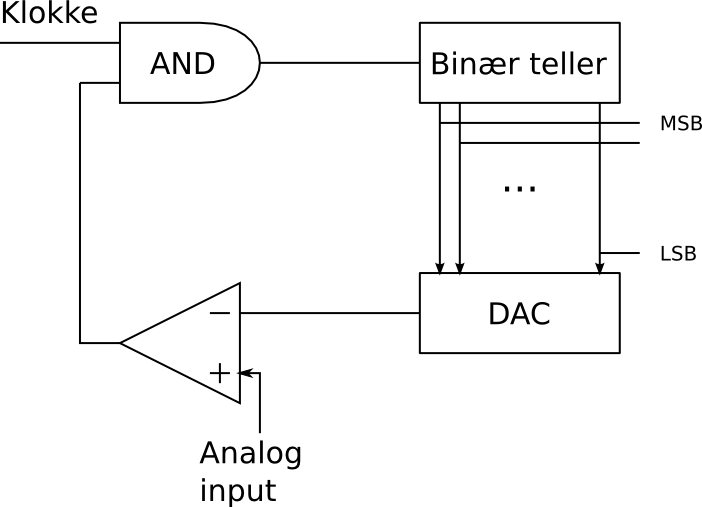
\includegraphics[width=0.67\textwidth]{./img/countingADC}
\end{figure}

For en verdi låst med Sample-Hold tikker klokka opp til riktig verdi.

\begin{figure}[H]
  \centering
  \caption{Output fra counting ADC}
  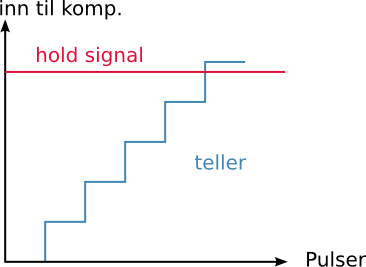
\includegraphics[width=0.5\textwidth]{./img/countingout}
\end{figure}

Skal man lese n-bit trenger konverteringen $2^n$ klokkepulser.
